\chapter{\label{chap:intro}Metodologia de Pesquisa}

A metodologia de pesquisa escolhida para este trabalho, é composta de um revisão da literatura já elaborada por Steglich e colegas \cite{caio2019} e de uma \textit{survey} que ainda será realizada. Para Ktichen end Pfleeger \cite{pfleeger2001principles} uma \textit{survey} consiste em sistema de coleta de dados e informações objetivando decifrar conhecimentos e práticas adotadas pelos sujeitos da pesquisa.
   
As etapas que compõe uma pesquisa \textit{survey} são:  definição do objetivo da pesquisa, definição da população e da amostra, elaboração do questionário, coleta de dados, processamento dos dados, análise dos dados e divulgação dos resultados \cite{vieira2010dicionario}.

\begin{figure}
    \centering
    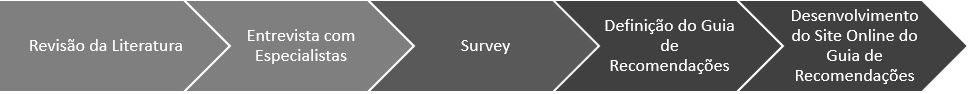
\includegraphics[scale=0.66]{fig/processo-metodologia.JPG}
    \caption{Metodologia de Pesquisa}
    \label{fig:my_label}
\end{figure}

\subsubsection{\textbf{Etapa 1 - Revisão da Literatura}}

%Pretendeu-se aprofundar o conhecimento na literatura de segurança em Ecossistemas de Software Móvel(ECOSM) e também em controles presentes na ISO 27002 utilizando como base a revisão da literatura feita por Steglich e colegas \cite{caio2019} que teve como objetivo identificar quais controles da ISO 27001 estão presentes na literatura de ECOSM, buscando verificar evidências sobre como eles são usados e o que a literatura relata sobre esses controles. O resultado do estudo mostrou que apenas 34 dos 114 controles da ISO 27001 estavam presentes na literatura de ECOSM e que apenas 2 de um total de 14 seções tinham seus respectivos controles evidenciados na literatura de ECOSM . Essas seções são, políticas de segurança da informação e criptografia. A falta de literatura sobre a maioria dos controles da ISO 27002, motivou o desenvolvimento deste trabalho.

%como por exemplo, um guia de recomendações visando auxiliar desenvolvedores mobile,

%\textbf{Como ponto de partida utilizou-se o trabalho de Steglich e colegas \cite{caio2019} com  32 referências de publicações que discutem informações de segurança no nível organizacional na literatura MSECO.}

 A partir da ISO 27002 e do estudo de Steglich e colegas \cite{caio2019} foram realizadas discussões com três professores, para a filtragem de seções e controles que se enquadrassem no contexto de desenvolvimento de software móvel, com o objetivo de eliminar seções irrelevantes e manter as que estivessem de acordo.
 



\subsubsection{ Etapa 2 - \textit{Entrevista com Especialistas}}

Visando confirmar a relevância dos controles selecionados, presentes na ISO/IEC 27002, buscou-se estratégias para que de fato os controles selecionados fossem relevantes para a execução de uma \textit{survey} com desenvolvedores de software móveis. Para isso, usou-se a abordagem de Entrevista com Especialistas para avaliação dos controles selecionados previamente, conforme recomendado por Flick \cite{flick2018introduction}. O autor esclarece que entrevistar especialistas pode servir a três propósitos: i) para exploração, para orientação em um novo campo, a fim de auxiliar a geração de hipóteses; ii) pode ser usada para coletar informações de contexto complementando percepções provenientes da aplicação de outros métodos; ou iii) pode também ser usada para geração de teorias que visam desenvolver uma tipologia ou uma teoria sobre uma questão a partir da reconstrução do conhecimento de vários especialistas. Com base no que foi expressado pelo autor \cite{flick2018introduction}, as entrevistas com os especialistas sarão utilizadas com o propósito ii), de coletar informações com a finalidade de complementar as percepções a respeito dos controles presentes na ISO/IEC 27002 que foram selecionados previamente e revisar a sua relevância.


\subsubsection{\textbf{Etapa 3 - \textit{Survey}}} Definiu-se como objetivo de pesquisa, conhecer quais os controles da ISO 27002 são adotados por desenvolvedores de software mobile e quais são as dificuldades enfrentadas ao tentar adotá-los, além de propor recomendações de como sobrepor essas dificuldades.Para atingir o objetivo do trabalho os seguintes passos serão realizados:
\begin{itemize}
\item \textit{Construir instrumento de coleta:} Para elaborar o questionário serão considerados os resultados anteriores das entrevistas com especialistas. O perfil desejado inicialmente para a realização da pesquisa será de desenvolvedores de software mobile.Os tipos de questões a serem realizadas serão decidas após a entrevista com os especialista, que já está prevista.

\item \textit{Validação do questionário:} Será realizado um piloto do questionário com colegas de curso que entendem de desenvolvimento mobile.

%O questionários será validado com desenvolvedores mobile com experiência alguns anos de experiência. Será realizado um piloto do questionário com colegas de curso que entendem de desenvolvimento mobile

\item \textit{Aplicação do questionário:} Será selecionada aleatoriamente uma amostra da população de desenvolvedores Mobile sobre a qual será solicitada o preenchimento de um questionário pela internet em grupos de Facebook, LinkedIn ou Github que ainda será desenvolvido, com o objetivo de responder o problema de pesquisa.

\item \textit{Analisar resultados:} Com o resultado do questionário será feita a análise dos dados, contudo a técnica de análise estatística ainda não foi definida. 
\end{itemize}


\subsubsection{\textbf{Etapa 3 - Definição do Guia de Recomendações}}

Requisitos de segurança como confidencialidade, integridade são abstratos e suas aplicações necessitam de uma orientação para serem seguidos, para que seja possível atender aos requisitos. Com os resultados da \textit{survey} ira ser criado um guia de recomendações de boas práticas com objetivo de auxiliar desenvolvedores a adotarem os controles previstos na ISO 27002. 

No processo para a elaboração do guia de recomendações pretende-se desenvolver um critério para a categorização de cada uma das orientações. O principal objetivo por trás dessa classificação é preparar a base para expressar esses guias em uma linguagem formal e argumentar sobre sua satisfação \cite{zhioua2016security}.

\subsubsection{\textbf{Etapa 4 - Desenvolvimento do \textit{Site Online} do Guia de Recomendações}}
Nessa etapa será necessário definir um formato de \textit{site}, com isso será preciso definir uma tecnologia para a construção do guia. Com o site estabelecido será necessário atualizá-lo com as recomendações e validá-lo com profissionais da indústria.

O cronograma foi dividido entre os 2 semestres do ano de 2020, contemplando
a metodologia \textit{survey}. No primeiro semestre foi elaborada uma análise critica da ISO
27002 separando as seções que eram relevantes para o objetivo trabalho. No segundo
semestre as seções serão validadas com especialistas para elaborar a \textit{survey} que irá gerar
resultados para elaborar um site com recomendações de boas práticas.

% Please add the following required packages to your document preamble:
% \usepackage{multirow}
% \usepackage[normalem]{ulem}
% \useunder{\uline}{\ul}{}
\begin{table}[]
\begin{center}
\caption{\label{tab:tab3}Cronograma TCC 2}%
\begin{tabular}{|c|l|c|c|c|c|l|l|}
\hline
\multirow{2}{*}{ETAPA}                                                                  & \multicolumn{1}{c|}{\multirow{2}{*}{ATIVIDADE}}                                                     & \multicolumn{6}{c|}{TCC 2}                                                                                                                                                                         \\ \cline{3-8} 
                                                                                        & \multicolumn{1}{c|}{}                                                                               & Jul                                    & Ago                   & Set                   & Out                   & \multicolumn{1}{c|}{Nov}                & \multicolumn{1}{c|}{Dez}                \\ \hline
TCC 1                                                                                   & Entrega do TCC 1                                                                                    & ok                                     &                       &                       &                       & \multicolumn{1}{c|}{}                   & \multicolumn{1}{c|}{}                   \\ \hline
\multirow{4}{*}{\begin{tabular}[c]{@{}c@{}}Entrevista com\\  Especialista\end{tabular}} & Selecionar entrevistados                                                                            & ok                                      &                       &                       &                       & \multicolumn{1}{c|}{}                   & \multicolumn{1}{c|}{}                   \\ \cline{2-8} 
                                                                                        & Elaborar peguntas                                                                                   & x                                      &                       &                       &                       & \multicolumn{1}{c|}{}                   & \multicolumn{1}{c|}{}                   \\ \cline{2-8} 
                                                                                        & Entrevistar                                                                                         & x                                      &                       &                       &                       & \multicolumn{1}{c|}{}                   & \multicolumn{1}{c|}{}                   \\ \cline{2-8} 
                                                                                        & Validar Perguntas das Entrevistas                                                                   & x                                      &                       &                       &                       & \multicolumn{1}{c|}{}                   & \multicolumn{1}{c|}{}                   \\ \hline
\multirow{7}{*}{Survey}                                                                 & Elaborar questionário                                                                               & x                                      &                       &                       &                       & \multicolumn{1}{c|}{}                   & \multicolumn{1}{c|}{}                   \\ \cline{2-8} 
                                                                                        & validar questionário                                                                                & x                                      & \multicolumn{1}{l|}{} & \multicolumn{1}{l|}{} & \multicolumn{1}{l|}{} &                                         &                                         \\ \cline{2-8} 
                                                                                        & realizar piloto do questionário                                                                     & x                                      &                       & \multicolumn{1}{l|}{} & \multicolumn{1}{l|}{} &                                         &                                         \\ \cline{2-8} 
                                                                                        & identificar respondentes                                                                            &                                        & x                     & \multicolumn{1}{l|}{} & \multicolumn{1}{l|}{} &                                         &                                         \\ \cline{2-8} 
                                                                                        & Convidar participantes                                                                              &                                        & x                     & \multicolumn{1}{l|}{} & \multicolumn{1}{l|}{} &                                         &                                         \\ \cline{2-8} 
                                                                                        & Aplicar questionário                                                                                &                                        & x                     &                       & \multicolumn{1}{l|}{} &                                         &                                         \\ \cline{2-8} 
                                                                                        & Analisar resultado                                                                                  &                                        & x                     &                       & \multicolumn{1}{l|}{} &                                         &                                         \\ \hline
\multirow{6}{*}{\begin{tabular}[c]{@{}c@{}}Guia de\\  Recomendações\end{tabular}}       & definir um formato de site                                                                          &                                        &                       & x                     & \multicolumn{1}{l|}{} &                                         &                                         \\ \cline{2-8} 
                                                                                        & Aprender como gerar o site                                                                          &                                        &                       & x                     &                       &                                         &                                         \\ \cline{2-8} 
                                                                                        & Denifi/propor as recomendações                                                                      & \multicolumn{1}{l|}{}                  &                       & x                     &                       &                                         &                                         \\ \cline{2-8} 
                                                                                        & Atualizar o site com recomendações                                                                  & \multicolumn{1}{l|}{}                  &                       &                       & x                     &                                         &                                         \\ \cline{2-8} 
                                                                                        & \begin{tabular}[c]{@{}l@{}}Planejar avaliação do site\\ com profissionais da industria\end{tabular} & \multicolumn{1}{l|}{}                  &                       &                       & x                     &                                         &                                         \\ \cline{2-8} 
                                                                                        & \begin{tabular}[c]{@{}l@{}}Avaliar site com profissionais\\  da indústria\end{tabular}              & \multicolumn{1}{l|}{}                  &                       &                       &                       &                                         &                                         \\ \hline
\multirow{2}{*}{TCC 2}                                                                  & \multicolumn{1}{c|}{\multirow{2}{*}{Escrever resultados}}                                           & \multicolumn{1}{l|}{\multirow{2}{*}{}} & \multirow{2}{*}{x}    & \multirow{2}{*}{x}    & \multirow{2}{*}{x}    & \multicolumn{1}{c|}{\multirow{2}{*}{x}} & \multicolumn{1}{c|}{\multirow{2}{*}{x}} \\
                                                                                        & \multicolumn{1}{c|}{}                                                                               & \multicolumn{1}{l|}{}                  &                       &                       &                       & \multicolumn{1}{c|}{}                   & \multicolumn{1}{c|}{}                   \\ \hline
\end{tabular}
\end{center}
\end{table}